\chapter{RSA - Model}
\label{chapter:rsa-model}
Human cognition allows us to pragmatically infer the meaning of utterances even beyond literal semantic meaning.
One common example is given by "scalar implicatures" as triggered by the word \textit{some} in "I ate some of your cookies". Taken literally, \textit{some} is compatible with \textit{all}, nevertheless we often infer that the speaker meant "some but not all". This is because we are assuming that the speaker wants to be informative. In a possible world where the speaker ate all cookies, he would have said "I ate all of your cookies", because this would give more information for the listener. By taking into account the speaker's alternative utterances and the use of them in various possible worlds, listeners implicitly entertain a model of the speaker's utterance choice. This model can be used for reasoning about the meaning of an utterance, which enables listeners "to make more informed interpretive choices than would be possible if they simply updated their information states with the information that the utterance's semantic interpretation is true." \citep{lassiter2017adjectival}\\

A formal model of language comprehension, that takes into account the listener's intuitive theory of how the speaker chooses words, is given through a "Rational Speech Act model" (RSA model), used by \cite{goodman2013knowledge}.
This chapter will introduce the main components of the RSA model as well as the underlying idea of probabilistic recursive reasoning. Afterwards, a new sort of extension to the RSA model is presented and evaluated.

\section{Main idea of RSA and Bayes' Theorem}
\begin{quote}
"RSA models language use as a recursive process in which
speakers and listeners reason about each other to enrich the literal semantics of their language.
This increases the efficiency and reliability of their communication compared to what more
purely literal agents can achieve." \citep{monroe2015learning}
\end{quote}
As mentioned in the citation above, the RSA model provides a description of an agent's language understanding and language production.
Numerous variations and applications of this model have been used for predicting phenomena like "scalar implicatures" or non-literal understanding of number words \citep[see][]{goodman2013knowledge, kao2014nonliteral}. By now, the RSA model has mostly been used to model language behavior by assuming a fixed set of utterances and their semantics. This set of semantics is given by a (hand-built) lexicon. Before introducing the concrete implementation of an agent's inference strategies, the following paragraph will give a brief explanation of \textbf{Bayes' Theorem}, which will be used in the description later.
Bayesian inference in general is introduced by \cite{lassiter2017adjectival}, 
therefore I will focus on the following theorem:
\begin{theorem}[Bayes' Theorem]
$P(B \mid A) \propto P(A \mid B) \cdot Pr(B)$
\end{theorem}
It provides a rather simple formula for calculating \textit{a-posteriori}-probabilities (the probability of hypothesis $B$ to be true, after seeing some event $A$). For this you need to know the conditional probability of $A$ being true, given hypothesis $B$, as well as the \textit{a-priori}-probability of $B$ being true (the probability of $B$ being true, without considering any further indications). Note that there is no equality sign. For equality, the right side of the formula must be derived by the marginal probability $P(A)$. While $P(A)$ is generally hard to compute, proportionality is assumed instead of equality ($A \propto B$ means that $A$ is directly proportional to $B$). This allows to omit the normalizing constant $P(A)$ and still obtain similar results. This inference technique is used for modeling the language behavior of an agent, as described in the following section.

\section{Inference strategies in RSA}
Consider a communication situation like the one described in section \ref{sec:egt}. A non-pragmatic "literal listener $L_0$" simply updates it's prior information state on the truth-value of an utterance $m$. $L_0$ infers a world state $w$ (e.g. the height of a person) after hearing a message $m$ (e.g. \textit{tall}), updating his prior information state $Pr(w)$ using an instance of Bayes Theorem. The formula is given in Eq.\ref{eq:L0-rsa} below.
\begin{equation}
\label{eq:L0-rsa}
P_{L0}(w \mid m) \propto \llbracket m \rrbracket^w \cdot Pr(w) 
\end{equation}
The "meaning-function" $\llbracket m \rrbracket^w$ takes on values between zero and one, representing the degree to which a message $m$ is true in world state $w$. Therefore it can also be formulated as $P(m $ is true $ \mid w)$.
"$Pr(w)$ specifies $L_1$'s background knowledge about answers to the QUD. For
example, if the QUD is 'How tall is Al?' and $L_1$ knows only that Al is an adult man,
then $Pr(w)$ is an estimate of the distribution of heights among adult men" \citep{lassiter2013context}. The presented model of a literal listener is used to model rational/informative speaker behavior as described in the following paragraph.\\

An informative speaker chooses an utterance $m$ from a finite set of alternatives $M$. The choice is made by reasoning about how a hypothetical literal listener $L_0$ would understand an utterance in the present circumstances.
In general, for capturing a speaker's motivation to be informative, the informative content for the listener is to be maximized. A false utterance will not provide any informative content and therefore is not likely to be chosen by a rational speaker. In order to model informative behavior mathematically, the utility $U$ of a message $m$ for the speaker $S_1$ is defined to be proportional to the informative content/informativity for the listener, who is reasoning about the true answer (the true world state) $w$.
The definition of informativity used here is given by \cite{lassiter2013context}:\begin{quote}
"Informativity is quantified as negative surprisal (positive log probability) of the true answer in the posterior, assuming that the utterance is true under the relevant parametrization."
\end{quote}
Negative surprisal is to be understood here as the amount of information that $L0$ would still not know about $w$, after hearing message $m$:
\begin{equation}
U_{S1}(m, w) = log(P_{L0}(w \mid m))
\end{equation}
After applying a soft-max choice rule to the utility function (which means that the probability of making a certain choice increases with its utility), the informative speaker model is obtained. The probability of choosing a certain utterance $m$, given an observed world state $w$, is given in Eq.\ref{eq:S1-rsa}.
The formula contains a "rationality parameter" $\alpha$ > 0. It determines how closely the stochastic choice approximates the deterministic utility-maximization i.e. the deviation from optimality. The effect of this parameter on the actual inference strategies is discussed later in this chapter. The notion of "recursive reasoning" is derived from the assumption that listeners and speakers maintain probabilistic models about each others behavior that drive pragmatic language use.
This idea of recursive reasoning is embedded in the formalization of the inference behavior of a pragmatic listener $L_1$. Messages are interpreted by reasoning about the speaker-model, which itself contains reasoning about a listener-model. This is done by taking into account what the speaker is likely to say, given a certain observation $w$ as well as the prior probability of $w$, as given in Eq.\ref{eq:L1-rsa}:
\begin{align}
\label{eq:S1-rsa}
P_{S_1}(m \mid w) &\propto exp(\alpha \cdot U_{S1}(m,w))\\
P_{L_1}(w \mid m) &\propto P_{S_1}(m \mid w) \cdot Pr(w)
\label{eq:L1-rsa}
\end{align}
The described models of pragmatic language understanding ($P_{L_1}$) and informative language use ($P_{S_1}$) will now be used for specifying language behavior of artificial agents. An innovative extension to the model is presented, that allows to take into account different underlying semantics.\\
The extended model will later be used for simulating a population of rational agents and their respective language use/understanding along Gricean lines. 
Chapter 5 examines which strategies/semantics are optimal, assuming that the agents behave according to the RSA model. This is a rather new application of the model.

\section{Agent types}
What properties define an agent in this scenario? An agent is fully described by its underlying \textit{type} $t$. A \textit{type} consists of three parameters:
$\mu, \sigma$ and $\alpha$. The following sections will describe the speaker and listener behavior as a mapping from their type $t$ to the respective inferences, according to the RSA model.\\

The parameters $\mu$ and $\sigma$ feed into a Gaussian distribution that represents the belief about the semantic threshold $\theta$, after which to use \textit{tall} (or \textit{short} likewise). Figure \ref{subfig:p-crisp} shows an exact belief about the value of $\theta$, with $P(\theta \mid \mu = 1.5, \sigma=0.001)$. This type would result in a crisp interpretation/a crisp meaning function, as in Fig.\ref{subfig:cdf-crisp}. On the other hand, a bigger $\sigma$ leads to a more vague interpretation/meaning function, see Fig.\ref{subfig:p-vague} (with $P(\theta \mid \mu=1.5, \sigma=0.2)$ and Fig.\ref{subfig:cdf-vague}.\\

Parameter $\alpha$ models an agent's "degree of rationality"/"optimality".
A more detailed explanation of the type's effect on the resulting inference strategies is given in the following sections, where the original formulas of the RSA model are extended by the type of an agent.

\section{Literal listener $L_0$}
%% L0 was displayed wrong because of discrete world Prior with 0.1-steps.
%% Set the discretization-steps to 0.00001, and the result looks as expected.
\begin{figure}[h]
 	\centering
 	\subfloat[L0-type: $\mu=1.5,\, \sigma=0.0001,\, \alpha=10$\label{subfig-1:L0_crisp}]{
 	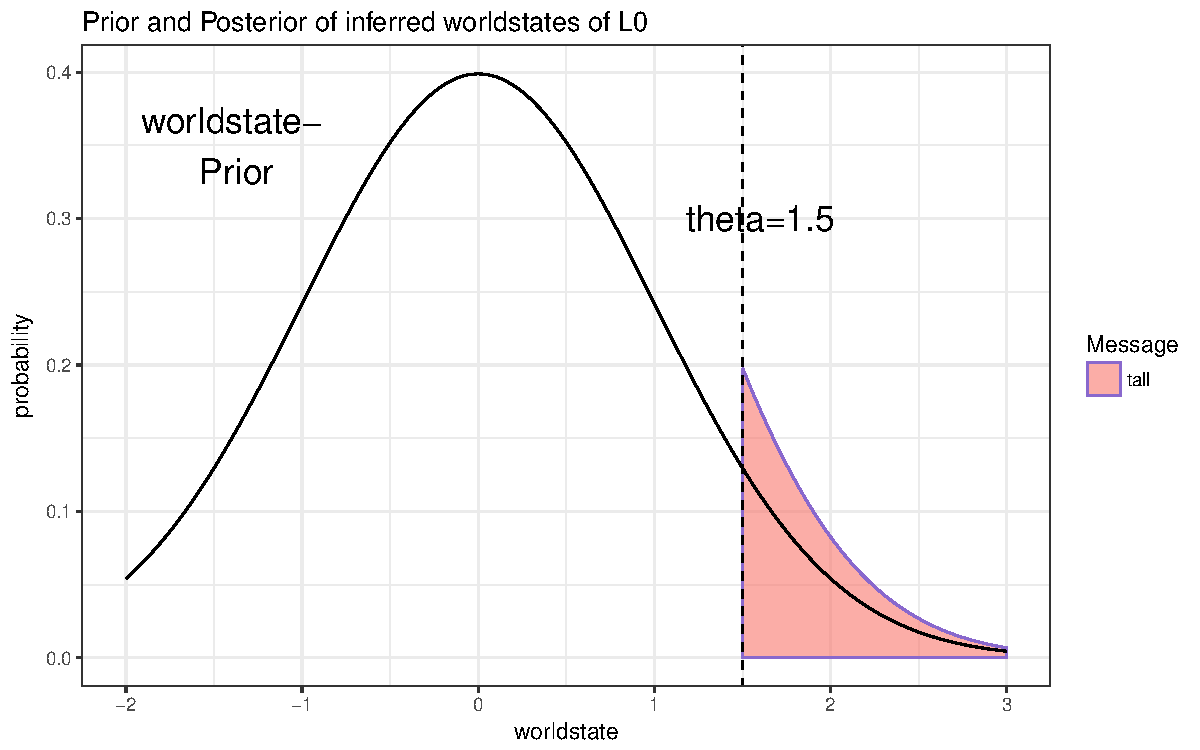
\includegraphics[width=0.5\textwidth]{L0-schematic-crisp.pdf}
 	} 	
 	\subfloat[L0-type: $\mu=1.5,\, \sigma=0.3,\, \alpha=10$\label{subfig-1:L0_vague}]{
 	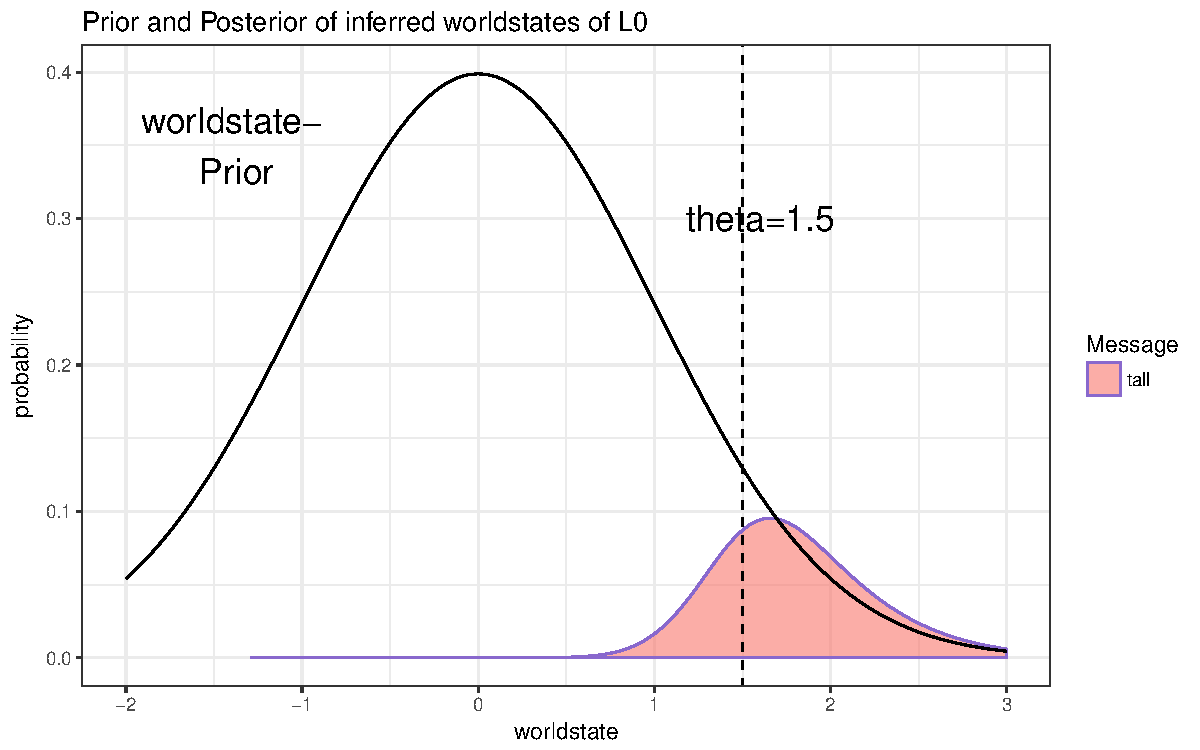
\includegraphics[width=0.5\textwidth]{L0-schematic-vague.pdf}
 	}
 \caption{Literal listener posteriors for a crisp and vague type.}
 \label{figure:L0-posterior}
\end{figure}
A literal listener is considered to interpret an utterance by its literal meaning. The interpretation results in a belief about the world state that was described by the speaker i.e. an answer to the current question under discussion. 
This might be e.g. the number of cookies eaten when your friend says he "ate some of the cookies" and is represented through a probability distribution over possible world states.
Another example for inference over world states can be the height of people, after hearing the sentence "Marc is tall".\\

By extending the original model by an agent's type $t = \big[ \mu, \sigma, \alpha\big]$, the resulting definition of the literal listener $L_0$ looks like this:
\begin{equation}
P_{L0}(w \mid m , \big[ \mu, \sigma, \alpha\big]) = \llbracket m \rrbracket^{w,\mu,\sigma} \cdot Pr(w) 
\end{equation}
A possible implementation of the meaning function $\llbracket m \rrbracket$ was given in section 2.3. The type-parameters $\mu$ and $\sigma$ model the distribution $P(\theta)$ and the literal meaning of an utterance $m$ under $w$ is derived by $P(\theta)$ in the following way:
\begin{equation}
\llbracket m \rrbracket^{w,\mu,\sigma} = P(m \, \textsf{is true} \mid w, \mu, \sigma) = \Phi(P(\theta \mid \mu, \sigma))(w)
\label{eq:meaning-func}
\end{equation}
This truth-functional meaning function is used by $L_0$. For the simulation in chapter \ref{chapter:simulation}, I will go further into detail on the implementation of the literal meaning function for the alternatives \{\textit{short}, \textit{not-short}, \textit{not-tall}, \textit{tall}\}, following Eq.\ref{eq:meaning-func}.\\

Using Bayesian inference and conditioning the prior information state on the truth of message $m$ results in a posterior probability distribution over possible world states, i.e. an interpretation of $m$. Different types result in different interpretations, as visualized in Figure \ref{figure:L0-posterior}, with the example $m = tall$. 
The strategy of $L_0$ is a mapping from its type to an interpretation of message $m$. 
Note, that $\alpha$ does not occur in the definition of the literal listener $L_0$, but it will be explained in the next section. 

\section{Informative Speaker $S_1$}
\begin{figure}[h]
 	\centering
 	\subfloat[S1-type: $\mu=1.5,\, \sigma=0.3,\, \alpha=1$\label{subfig-1:S1_naive}]{
 	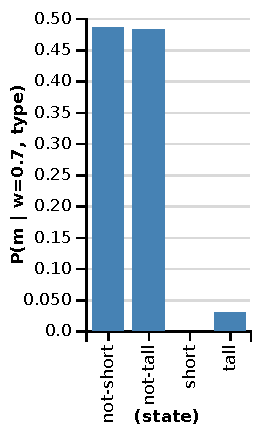
\includegraphics[width=0.35\textwidth]{S1-alpha1.pdf}
 	} 	
	\qquad \qquad
 	\subfloat[S1-type: $\mu=1.5,\, \sigma=0.3,\, \alpha=100$\label{subfig-1:S1_rational}]{
 	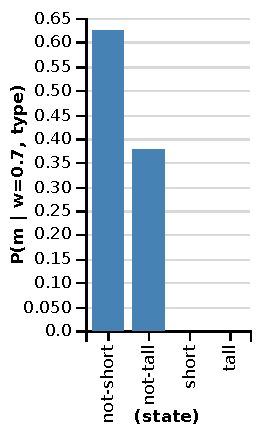
\includegraphics[width=0.35\textwidth]{S1-alpha100.pdf}
 	}
 \caption{Speaker choices of a naive and rational type, for $w=0.7$}
 \label{figure:S1-posterior}
\end{figure}
In this framework, the speaker is considered to select utterances that are informative relative to the current question under discussion. The choice of an utterance is made with respect to the alternatives and is now extended to be also dependent on type $t = \big[ \mu, \sigma, \alpha\big]$:
\begin{align}
P_{S1}(m \mid w, \big[ \mu, \sigma, \alpha\big]) &\propto exp(\alpha \cdot U_{S1}(m,w, \big[ \mu, \sigma, \alpha\big]))\\
U_{S1}(m, w, \big[ \mu, \sigma, \alpha\big]) &= log(P_{L0}(w \mid m, \big[ \mu, \sigma, \alpha\big]))
\end{align}
As mentioned before, one property of an agent's  strategy is its "degree of rationality", which is modeled through the parameter $\alpha$. $\alpha=0$ means, the choice of the message is made completely random, as a uniform draw from $M$. $\alpha=\infty$ means, the speaker is completely rational in the sense, that the choice truly optimizes the utility. This effect is visualized in Fig.\ref{figure:S1-posterior}. The message choices for describing the world state $w=0.7$ are shown, for a naive speaker (with $\alpha=1$) and a rational speaker (with $\alpha=100$). It can be seen that for a small $\alpha$, there is no clear preference for either of the messages. A more rational agent with a bigger $\alpha$ shows clearer preferences. This effect will get clearer when looking at the posteriors of $L_1$, in the next section.

\section{Pragmatic listener $L_1$}
\begin{figure}[h]
 	\centering
 	\subfloat[L1-type: $\mu=0.8,\, \sigma=0.01,\, \alpha=1$\label{subfig-1:L1_crisp_1}]{
 	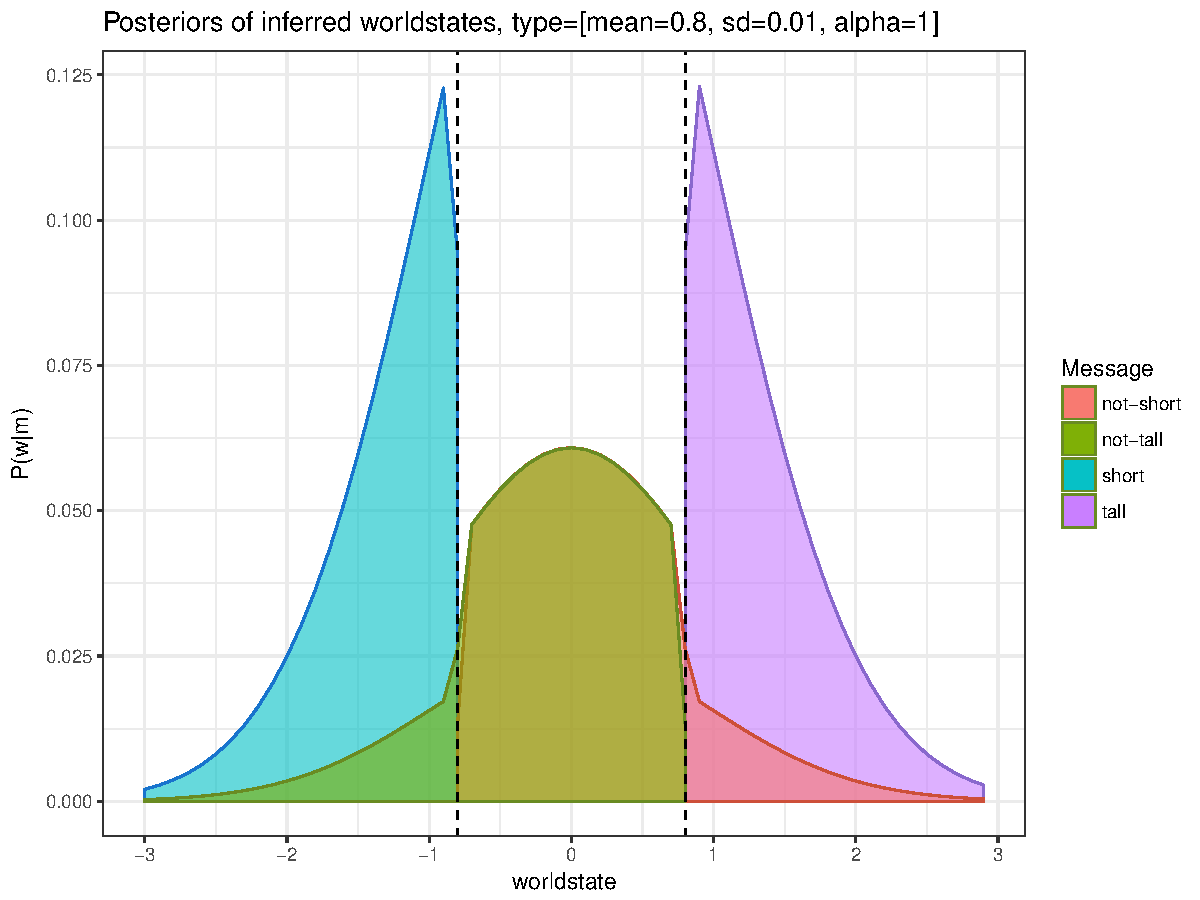
\includegraphics[width=0.5\textwidth]{L1_crisp_alpha=1.pdf}
 	} 	
 	\subfloat[L1-type:$\mu=0.8,\, \sigma=0.01,\, \alpha=50$\label{subfig-1:L1_crisp_50}]{
 	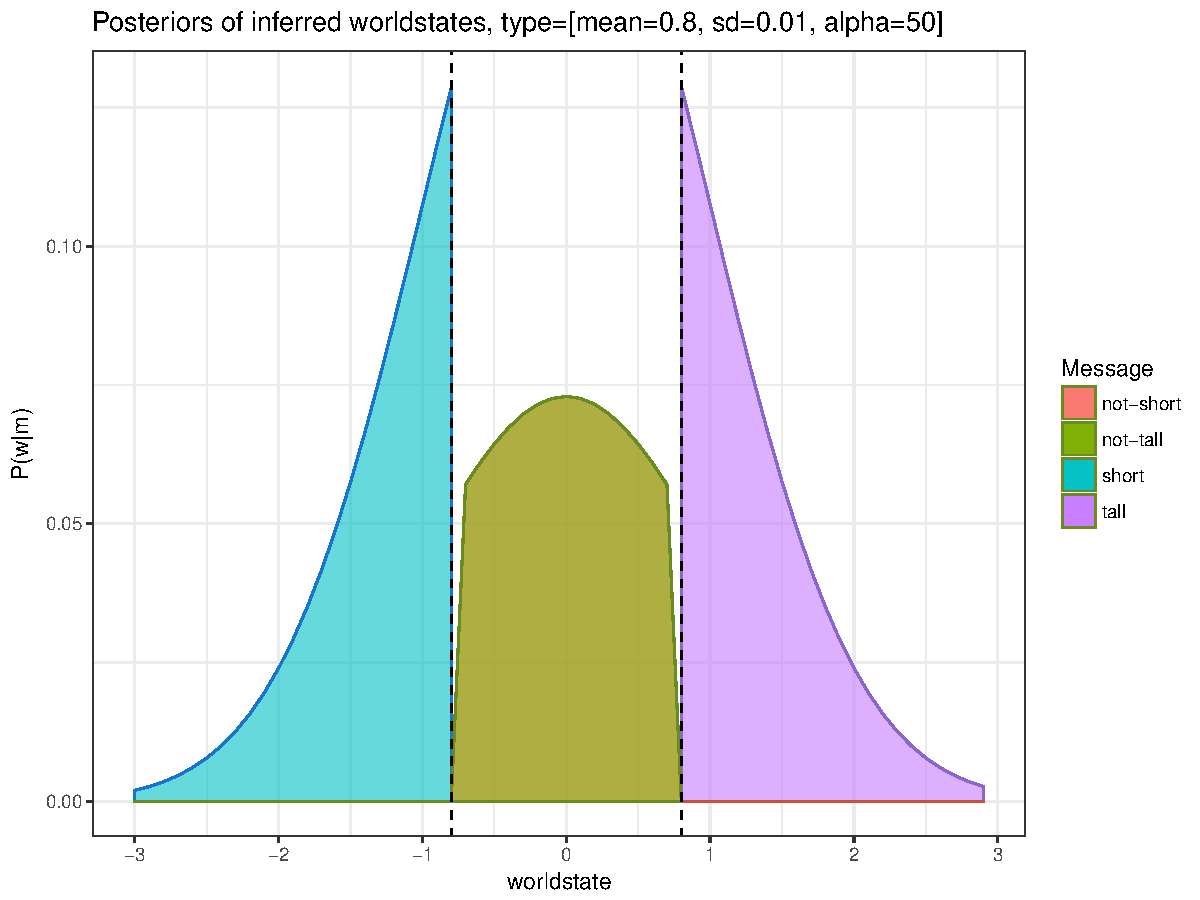
\includegraphics[width=0.5\textwidth]{L1_crisp_alpha=50.pdf}
 	}
 	\\
 	\subfloat[L1-type:$\mu=0.8,\, \sigma=0.5,\, \alpha=1$\label{subfig-1:L1_vague_1}]{
    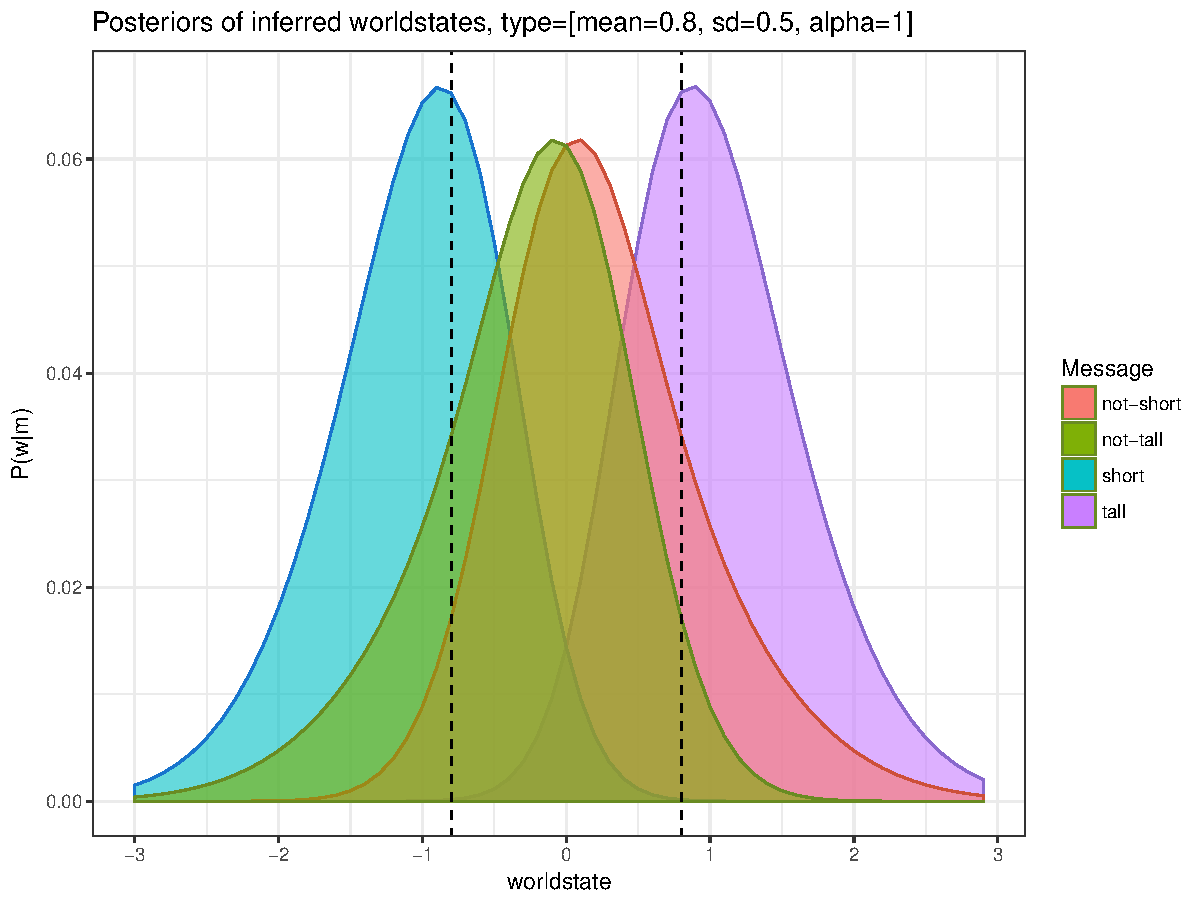
\includegraphics[width=0.5\textwidth]{L1_opt_alpha=1.pdf}
 	}
 	\subfloat[L1-type:$\mu=0.8,\, \sigma=0.5,\, \alpha=50$\label{subfig-1:L1_vague50}]{
    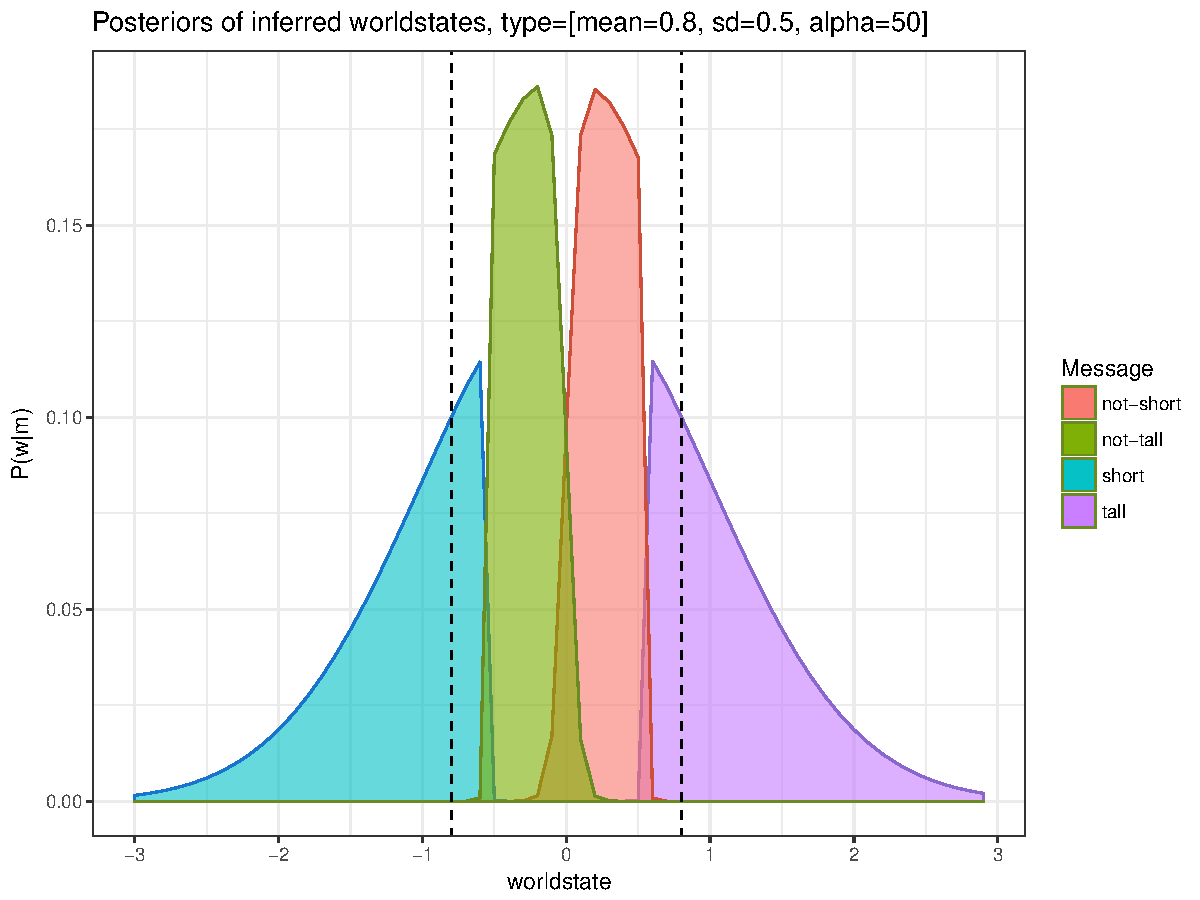
\includegraphics[width=0.5\textwidth]{L1_opt_alpha=50.pdf}
 	}
 \caption{Listener posteriors for different types}
 \label{figure:L1-posterior}
\end{figure}
The extension of $L_1$ is rather straightforward:
\begin{equation}
P_{L_1}(w \mid m, \big[ \mu, \sigma, \alpha\big]) \propto P_{S_1}(m \mid w, \big[ \mu, \sigma, \alpha\big]) \cdot Pr(w)
\end{equation}
Parameters $\mu$ and $\sigma$ are passed through to the level of $L_0$, where they are used for resolving the literal meaning of an utterance. Parameter $\alpha$ is passed trough to the level of $L_1$, where it determines the "optimality" of an agent's choice. Different posterior distributions for different listener types are presented in Figure \ref{figure:L1-posterior}. The effect of the parameters $\alpha$ and $\sigma$ on the resulting strategies is discussed below.\\

The effect of a small alpha ($\alpha=1$, Figures \ref{subfig-1:L1_crisp_1} and \ref{subfig-1:L1_vague_1}) can be found in the left column, a bigger alpha ($\alpha=50$, Figures \ref{subfig-1:L1_crisp_50} and \ref{subfig-1:L1_vague50}) in the right column. The first row shows a crisp listener strategy (type with $\mu=0.8$, $\sigma=0.01$ and $\alpha$ as described above), i.e. posterior probability distributions over inferred world states after hearing a certain utterance. The second row shows a vague listener type (type with $\mu=0.8$, $\sigma=0.5$ and $\alpha$ as described above). For the crisp type with $\sigma = 0.01$, the inferred meanings after the thresholds are quite clear, which is no surprise given the implemented semantics. What is more interesting, that in the area between the thresholds, it is completely unclear which interpretation choices will be made. The inferred probabilities over world states are very similar after hearing \textit{not-tall} or \textit{not-short}. This is also true for the naive vague type in Fig.\ref{subfig-1:L1_vague_1} with the difference that the inferred meaning of \textit{tall} and \textit{short} is very vague around the threshold.\\

Only for the rational vague strategy in Fig.\ref{subfig-1:L1_vague_1} we can observe clear and separate preferences over world states after hearing different messages. The state space has been partitioned into categories. \textit{Tall} is roughly interpreted as "taller than $\theta$", analogous to the meaning of \textit{short}. Being \textit{not-short} means "slightly taller than the norm" and \textit{not-tall} means "slightly smaller than the norm".
The ordering of the utterances' meaning is similar to the results of \cite{tesslernot}.
Figure \ref{figure:L1-posterior} nicely displays that the rational use of vague terms leads to a better understanding of the respective logical negations, while a rational crisp strategy lacks this feature.
